% !TEX root = ../thesis.tex

%=========================================================
\section{Atomic Contacts}
\label{sec:atomic-contacts}
%=========================================================

    \begin{wrapfigure}[13]{r}{40mm}
        \captionsetup{format=plain}%
        \centering
        \vspace{-1.5em}
        {
            \fontsize{7}{9}\selectfont
            \import{tunnelbarrier/samples}{AC.pdf_tex}
        }
        \vspace{-1.5em}
        \caption{
            SEM image of sample `AC'. $80\,\mathrm{nm}$ of Al.
        }
        \label{fig:ac:image-AC}
    \end{wrapfigure}

    Mesurements were performed on sample AC, shown in Fig \ref{fig:ac:image-AC}. Also known as PR-22e-09. Setup used as in Patrick Raif and Martin Presel. Data aquisition as described in Sec. \ref{sec:methods:ditigal}. All microwave irradiation experiments shown in this section are done in corporation with Patrikc Raif during his Master's Thesis.

    We did a lot of characterization of the unbroken device, shown in Patrick Raif. However no effects of microwave irradiation has been measured. 
    
    The samples gap and critical temperature are 
    \begin{align}
        \Delta_0 = 189(1)\,\mathrm{ueV}\, &&
        T_\mathrm{c} = 1.2\,\mathrm{K}\,.
    \end{align}
    The gap could be estimated by the fits, and their clustering value. Measurements in the tunnel limit, that could be fitted with the bcs theory confirm this gap. The critcal temperature is retrieved by a temperature study on the same caontact in the tunnel limit.
    
    The sample in the unbroken state was characterized with Patrick and is described in \cite{raif_electronic_2024}. The order parameter in the unbroken state were found to be
    \begin{align}
        I_\mathrm{c} = 10.0\,\mathrm{nA}\,, &&
        G_\mathrm{N} = 100.0\,G_0\,, &&
        \mu_0H_\mathrm{c} = 100\,\mathrm{mT}\,.
    \end{align}
    Critical- / Switching current and normal state conductance strongly depend the state of the break junction.

    %=========================================================
    \subsection{The Mesoscopic Pincode}
    \label{sec:ac:pincode}
    %=========================================================
    

    The mesoscopic pincode \(\{\tau_i\}\) describes the transmission eigenvalues of the atomic contact, as introduced in Sec.~\ref{subsec:quasi:meso}. Its channel-dependent MAR spectrum is discussed in Sec.~\ref{subsec:meso:mar}. I extracted the pincode using the fitting procedure described in Sec.~\ref{subsec:methods:digital:analysis}.

    After characterization of the unbroken sample, the break junction can be broken and atomic contacts might form. By measuring spectra over small changes in displacements, one can obtain the mesoscopic pincode.

    Figure \ref{fig:ac:pincode:fits} shows representative fits of taken I--V spectra at positions $\Delta x$. Those units are arbitrary motor positions and not calibrated. However i assume it as an proportional axis to the real displacement. For those fits I assume those values statically:
    \begin{align}
        T = 0\,\mathrm{K}\,, &&
        \gamma = 1\,\mathrm{neV}\,.
    \end{align}

    
    \begin{align}
        \Delta_0 = 188.5(5)\,\mathrm{ueV}\,, &&
        \sigma_V = 26(1)\,\mathrm{ueV}\,.
    \end{align}

    \begin{figure}[t]
        \centering
        \subfigure[
            \textit{I--V}
        ]{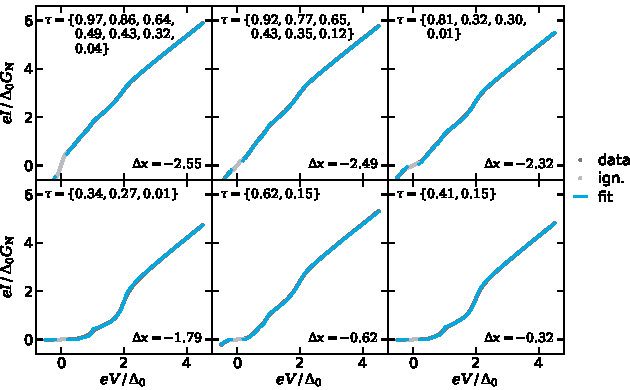
\includegraphics{atomic_contact/breaking/ivs.pdf}}
        \subfigure[
            \textit{dI--dV}
        ]{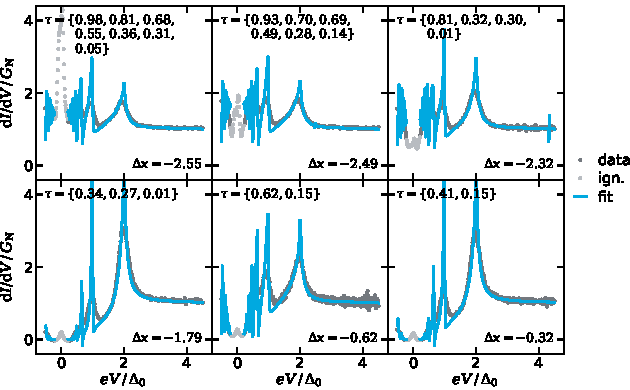
\includegraphics{atomic_contact/breaking/didvs.pdf}}        
        \caption{
            The retrieved pincode has an uncertainty of $0.01$, Since the preacalculated grid doesnt allow for higher resolution. Figure  show the results of all the taken ivs. We can observe the normal conductance and the contributions of single channels.
        }
        \label{fig:ac:pincode:fits}
    \end{figure}

    \begin{wrapfigure}[13]{r}{1.7in}
        \captionsetup{format=plain}%
        \centering
        % \vspace{-1.5em}
        \import{atomic_contact/breaking}{pincode.pgf}
        % \vspace{-1.5em}
        \caption{
            bla
        }
        \label{fig:ac:pincode}
    \end{wrapfigure}

    The retrieved pincode has an uncertainty of $0.01$, Since the preacalculated grid doesnt allow for higher resolution. Figure \ref{fig:ac:pincode} show the results of all the taken ivs. We can observe the normal conductance and the contributions of single channels.

    The normal conductance result in plateaus. However the last two plateus increase in conductance towards their end. From the single channels we see, that a single channel contribution rises and the other two channels lower their contribution, we attribute this to ...

    The full waterfall plot of this measurement is found in \ref{fig:ac:pincode:cal} and the corresponding simulation can be found in \ref{fig:ac:pincode:fit}.

    \transportlandscapefigure{atomic_contact/breaking}{cal}{
        bla blab la
    }{fig:ac:pincode:cal}

    \transportlandscapefigure{atomic_contact/breaking}{sim}{
        bla blab la
    }{fig:ac:pincode:sim}